\documentclass[1p]{elsarticle_modified}
%\bibliographystyle{elsarticle-num}

%\usepackage[colorlinks]{hyperref}
%\usepackage{abbrmath_seonhwa} %\Abb, \Ascr, \Acal ,\Abf, \Afrak
\usepackage{amsfonts}
\usepackage{amssymb}
\usepackage{amsmath}
\usepackage{amsthm}
\usepackage{scalefnt}
\usepackage{amsbsy}
\usepackage{kotex}
\usepackage{caption}
\usepackage{subfig}
\usepackage{color}
\usepackage{graphicx}
\usepackage{xcolor} %% white, black, red, green, blue, cyan, magenta, yellow
\usepackage{float}
\usepackage{setspace}
\usepackage{hyperref}

\usepackage{tikz}
\usetikzlibrary{arrows}

\usepackage{multirow}
\usepackage{array} % fixed length table
\usepackage{hhline}

%%%%%%%%%%%%%%%%%%%%%
\makeatletter
\renewcommand*\env@matrix[1][\arraystretch]{%
	\edef\arraystretch{#1}%
	\hskip -\arraycolsep
	\let\@ifnextchar\new@ifnextchar
	\array{*\c@MaxMatrixCols c}}
\makeatother %https://tex.stackexchange.com/questions/14071/how-can-i-increase-the-line-spacing-in-a-matrix
%%%%%%%%%%%%%%%

\usepackage[normalem]{ulem}

\newcommand{\msout}[1]{\ifmmode\text{\sout{\ensuremath{#1}}}\else\sout{#1}\fi}
%SOURCE: \msout is \stkout macro in https://tex.stackexchange.com/questions/20609/strikeout-in-math-mode

\newcommand{\cancel}[1]{
	\ifmmode
	{\color{red}\msout{#1}}
	\else
	{\color{red}\sout{#1}}
	\fi
}

\newcommand{\add}[1]{
	{\color{blue}\uwave{#1}}
}

\newcommand{\replace}[2]{
	\ifmmode
	{\color{red}\msout{#1}}{\color{blue}\uwave{#2}}
	\else
	{\color{red}\sout{#1}}{\color{blue}\uwave{#2}}
	\fi
}

\newcommand{\Sol}{\mathcal{S}} %segment
\newcommand{\D}{D} %diagram
\newcommand{\A}{\mathcal{A}} %arc


%%%%%%%%%%%%%%%%%%%%%%%%%%%%%5 test

\def\sl{\operatorname{\textup{SL}}(2,\Cbb)}
\def\psl{\operatorname{\textup{PSL}}(2,\Cbb)}
\def\quan{\mkern 1mu \triangleright \mkern 1mu}

\theoremstyle{definition}
\newtheorem{thm}{Theorem}[section]
\newtheorem{prop}[thm]{Proposition}
\newtheorem{lem}[thm]{Lemma}
\newtheorem{ques}[thm]{Question}
\newtheorem{cor}[thm]{Corollary}
\newtheorem{defn}[thm]{Definition}
\newtheorem{exam}[thm]{Example}
\newtheorem{rmk}[thm]{Remark}
\newtheorem{alg}[thm]{Algorithm}

\newcommand{\I}{\sqrt{-1}}
\begin{document}

%\begin{frontmatter}
%
%\title{Boundary parabolic representations of knots up to 8 crossings}
%
%%% Group authors per affiliation:
%\author{Yunhi Cho} 
%\address{Department of Mathematics, University of Seoul, Seoul, Korea}
%\ead{yhcho@uos.ac.kr}
%
%
%\author{Seonhwa Kim} %\fnref{s_kim}}
%\address{Center for Geometry and Physics, Institute for Basic Science, Pohang, 37673, Korea}
%\ead{ryeona17@ibs.re.kr}
%
%\author{Hyuk Kim}
%\address{Department of Mathematical Sciences, Seoul National University, Seoul 08826, Korea}
%\ead{hyukkim@snu.ac.kr}
%
%\author{Seokbeom Yoon}
%\address{Department of Mathematical Sciences, Seoul National University, Seoul, 08826,  Korea}
%\ead{sbyoon15@snu.ac.kr}
%
%\begin{abstract}
%We find all boundary parabolic representation of knots up to 8 crossings.
%
%\end{abstract}
%\begin{keyword}
%    \MSC[2010] 57M25 
%\end{keyword}
%
%\end{frontmatter}

%\linenumbers
%\tableofcontents
%
\newcommand\colored[1]{\textcolor{white}{\rule[-0.35ex]{0.8em}{1.4ex}}\kern-0.8em\color{red} #1}%
%\newcommand\colored[1]{\textcolor{white}{ #1}\kern-2.17ex	\textcolor{white}{ #1}\kern-1.81ex	\textcolor{white}{ #1}\kern-2.15ex\color{red}#1	}

{\Large $\underline{12a_{0530}~(K12a_{0530})}$}

\setlength{\tabcolsep}{10pt}
\renewcommand{\arraystretch}{1.6}
\vspace{1cm}\begin{tabular}{m{100pt}>{\centering\arraybackslash}m{274pt}}
\multirow{5}{120pt}{
	\centering
	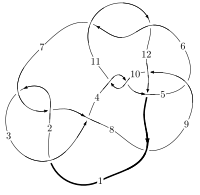
\includegraphics[width=112pt]{../../../GIT/diagram.site/Diagrams/png/1331_12a_0530.png}\\
\ \ \ A knot diagram\footnotemark}&
\allowdisplaybreaks
\textbf{Linearized knot diagam} \\
\cline{2-2}
 &
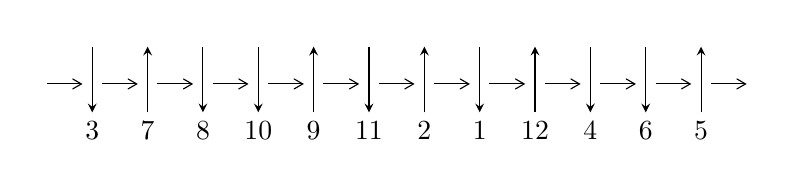
\begin{tikzpicture}[x=20pt, y=17pt]
	% nodes
	\node (C0) at (0, 0) {};
	\node (C1) at (1, 0) {};
	\node (C1U) at (1, +1) {};
	\node (C1D) at (1, -1) {3};

	\node (C2) at (2, 0) {};
	\node (C2U) at (2, +1) {};
	\node (C2D) at (2, -1) {7};

	\node (C3) at (3, 0) {};
	\node (C3U) at (3, +1) {};
	\node (C3D) at (3, -1) {8};

	\node (C4) at (4, 0) {};
	\node (C4U) at (4, +1) {};
	\node (C4D) at (4, -1) {10};

	\node (C5) at (5, 0) {};
	\node (C5U) at (5, +1) {};
	\node (C5D) at (5, -1) {9};

	\node (C6) at (6, 0) {};
	\node (C6U) at (6, +1) {};
	\node (C6D) at (6, -1) {11};

	\node (C7) at (7, 0) {};
	\node (C7U) at (7, +1) {};
	\node (C7D) at (7, -1) {2};

	\node (C8) at (8, 0) {};
	\node (C8U) at (8, +1) {};
	\node (C8D) at (8, -1) {1};

	\node (C9) at (9, 0) {};
	\node (C9U) at (9, +1) {};
	\node (C9D) at (9, -1) {12};

	\node (C10) at (10, 0) {};
	\node (C10U) at (10, +1) {};
	\node (C10D) at (10, -1) {4};

	\node (C11) at (11, 0) {};
	\node (C11U) at (11, +1) {};
	\node (C11D) at (11, -1) {6};

	\node (C12) at (12, 0) {};
	\node (C12U) at (12, +1) {};
	\node (C12D) at (12, -1) {5};
	\node (C13) at (13, 0) {};

	% arrows
	\draw[->,>={angle 60}]
	(C0) edge (C1) (C1) edge (C2) (C2) edge (C3) (C3) edge (C4) (C4) edge (C5) (C5) edge (C6) (C6) edge (C7) (C7) edge (C8) (C8) edge (C9) (C9) edge (C10) (C10) edge (C11) (C11) edge (C12) (C12) edge (C13) ;	\draw[->,>=stealth]
	(C1U) edge (C1D) (C2D) edge (C2U) (C3U) edge (C3D) (C4U) edge (C4D) (C5D) edge (C5U) (C6U) edge (C6D) (C7D) edge (C7U) (C8U) edge (C8D) (C9D) edge (C9U) (C10U) edge (C10D) (C11U) edge (C11D) (C12D) edge (C12U) ;
	\end{tikzpicture} \\
\hhline{~~} \\& 
\textbf{Solving Sequence} \\ \cline{2-2} 
 &
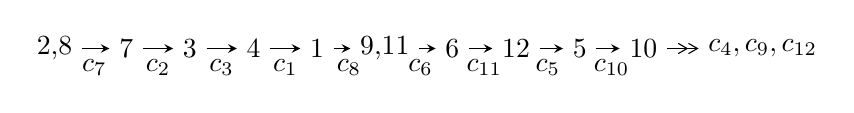
\begin{tikzpicture}[x=23pt, y=7pt]
	% node
	\node (A0) at (-1/8, 0) {2,8};
	\node (A1) at (1, 0) {7};
	\node (A2) at (2, 0) {3};
	\node (A3) at (3, 0) {4};
	\node (A4) at (4, 0) {1};
	\node (A5) at (81/16, 0) {9,11};
	\node (A6) at (49/8, 0) {6};
	\node (A7) at (57/8, 0) {12};
	\node (A8) at (65/8, 0) {5};
	\node (A9) at (73/8, 0) {10};
	\node (C1) at (1/2, -1) {$c_{7}$};
	\node (C2) at (3/2, -1) {$c_{2}$};
	\node (C3) at (5/2, -1) {$c_{3}$};
	\node (C4) at (7/2, -1) {$c_{1}$};
	\node (C5) at (9/2, -1) {$c_{8}$};
	\node (C6) at (45/8, -1) {$c_{6}$};
	\node (C7) at (53/8, -1) {$c_{11}$};
	\node (C8) at (61/8, -1) {$c_{5}$};
	\node (C9) at (69/8, -1) {$c_{10}$};
	\node (A10) at (11, 0) {$c_{4},c_{9},c_{12}$};

	% edge
	\draw[->,>=stealth]	
	(A0) edge (A1) (A1) edge (A2) (A2) edge (A3) (A3) edge (A4) (A4) edge (A5) (A5) edge (A6) (A6) edge (A7) (A7) edge (A8) (A8) edge (A9) ;
	\draw[->>,>={angle 60}]	
	(A9) edge (A10);
\end{tikzpicture} \\ 

\end{tabular} \\

\footnotetext{
The image of knot diagram is generated by the software ``\textbf{Draw programme}" developed by Andrew Bartholomew(\url{http://www.layer8.co.uk/maths/draw/index.htm\#Running-draw}), where we modified some parts for our purpose(\url{https://github.com/CATsTAILs/LinksPainter}).
}\phantom \\ \newline 
\centering \textbf{Ideals for irreducible components\footnotemark of $X_{\text{par}}$} 
 
\begin{align*}
I^u_{1}&=\langle 
41 u^{43}+223 u^{42}+\cdots+4 b+100,\;-57 u^{43}-353 u^{42}+\cdots+8 a-44,\;u^{44}+7 u^{43}+\cdots+68 u+8\rangle \\
I^u_{2}&=\langle 
9.53658\times10^{33} a^{5} u^{14}+2.36260\times10^{34} a^{4} u^{14}+\cdots-9.99117\times10^{34} a+8.92448\times10^{34},\\
\phantom{I^u_{2}}&\phantom{= \langle  }3 u^{14} a^4-10 u^{14} a^3+\cdots-4 a-5,\\
\phantom{I^u_{2}}&\phantom{= \langle  }u^{15}- u^{14}+4 u^{13}-3 u^{12}+8 u^{11}-6 u^{10}+10 u^9-7 u^8+8 u^7-6 u^6+6 u^5-4 u^4+4 u^3-2 u^2+2 u-1\rangle \\
I^u_{3}&=\langle 
-3 u^{25}- u^{24}+\cdots+b+2,\;u^{25}-2 u^{24}+\cdots+a-4,\;u^{26}+7 u^{24}+\cdots+3 u^2+1\rangle \\
\\
\end{align*}
\raggedright * 3 irreducible components of $\dim_{\mathbb{C}}=0$, with total 160 representations.\\
\footnotetext{All coefficients of polynomials are rational numbers. But the coefficients are sometimes approximated in decimal forms when there is not enough margin.}
\newpage
\renewcommand{\arraystretch}{1}
\centering \section*{I. $I^u_{1}= \langle 41 u^{43}+223 u^{42}+\cdots+4 b+100,\;-57 u^{43}-353 u^{42}+\cdots+8 a-44,\;u^{44}+7 u^{43}+\cdots+68 u+8 \rangle$}
\flushleft \textbf{(i) Arc colorings}\\
\begin{tabular}{m{7pt} m{180pt} m{7pt} m{180pt} }
\flushright $a_{2}=$&$\begin{pmatrix}0\\u\end{pmatrix}$ \\
\flushright $a_{8}=$&$\begin{pmatrix}1\\0\end{pmatrix}$ \\
\flushright $a_{7}=$&$\begin{pmatrix}1\\u^2\end{pmatrix}$ \\
\flushright $a_{3}=$&$\begin{pmatrix}u\\u^3+u\end{pmatrix}$ \\
\flushright $a_{4}=$&$\begin{pmatrix}- u^3\\u^3+u\end{pmatrix}$ \\
\flushright $a_{1}=$&$\begin{pmatrix}u^3\\u^5+u^3+u\end{pmatrix}$ \\
\flushright $a_{9}=$&$\begin{pmatrix}u^8+u^6+u^4+1\\u^{10}+2 u^8+3 u^6+2 u^4+u^2\end{pmatrix}$ \\
\flushright $a_{11}=$&$\begin{pmatrix}7.12500 u^{43}+44.1250 u^{42}+\cdots+65.2500 u+5.50000\\-\frac{41}{4} u^{43}-\frac{223}{4} u^{42}+\cdots-193 u-25\end{pmatrix}$ \\
\flushright $a_{6}=$&$\begin{pmatrix}\frac{67}{8} u^{43}+\frac{351}{8} u^{42}+\cdots-\frac{459}{4} u-16\\\frac{17}{4} u^{43}+\frac{161}{4} u^{42}+\cdots+\frac{1549}{2} u+101\end{pmatrix}$ \\
\flushright $a_{12}=$&$\begin{pmatrix}\frac{37}{8} u^{43}+\frac{215}{8} u^{42}+\cdots+\frac{167}{2} u+12\\-4 u^{43}-\frac{49}{2} u^{42}+\cdots-\frac{329}{2} u-21\end{pmatrix}$ \\
\flushright $a_{5}=$&$\begin{pmatrix}-\frac{59}{8} u^{43}-\frac{351}{8} u^{42}+\cdots-\frac{757}{4} u-23\\-\frac{3}{4} u^{43}-\frac{55}{4} u^{42}+\cdots-\frac{939}{2} u-63\end{pmatrix}$ \\
\flushright $a_{10}=$&$\begin{pmatrix}-0.875000 u^{43}+4.12500 u^{42}+\cdots+349.250 u+45.5000\\-\frac{37}{4} u^{43}-\frac{239}{4} u^{42}+\cdots-463 u-55\end{pmatrix}$\\&\end{tabular}
\flushleft \textbf{(ii) Obstruction class $= -1$}\\~\\
\flushleft \textbf{(iii) Cusp Shapes $= -7 u^{43}-47 u^{42}+\cdots-416 u-62$}\\~\\
\newpage\renewcommand{\arraystretch}{1}
\flushleft \textbf{(iv) u-Polynomials at the component}\newline \\
\begin{tabular}{m{50pt}|m{274pt}}
Crossings & \hspace{64pt}u-Polynomials at each crossing \\
\hline $$\begin{aligned}c_{1}\end{aligned}$$&$\begin{aligned}
&u^{44}+21 u^{43}+\cdots+112 u+64
\end{aligned}$\\
\hline $$\begin{aligned}c_{2},c_{7}\end{aligned}$$&$\begin{aligned}
&u^{44}+7 u^{43}+\cdots+68 u+8
\end{aligned}$\\
\hline $$\begin{aligned}c_{3}\end{aligned}$$&$\begin{aligned}
&u^{44}-7 u^{43}+\cdots-15900 u+2088
\end{aligned}$\\
\hline $$\begin{aligned}c_{4},c_{6},c_{10}\\c_{11}\end{aligned}$$&$\begin{aligned}
&u^{44}+20 u^{42}+\cdots+3 u+1
\end{aligned}$\\
\hline $$\begin{aligned}c_{5},c_{12}\end{aligned}$$&$\begin{aligned}
&u^{44}- u^{43}+\cdots-2 u+1
\end{aligned}$\\
\hline $$\begin{aligned}c_{8}\end{aligned}$$&$\begin{aligned}
&u^{44}+35 u^{43}+\cdots+9095124 u+659432
\end{aligned}$\\
\hline $$\begin{aligned}c_{9}\end{aligned}$$&$\begin{aligned}
&u^{44}+44 u^{43}+\cdots+819200 u+32768
\end{aligned}$\\
\hline
\end{tabular}\\~\\
\newpage\renewcommand{\arraystretch}{1}
\flushleft \textbf{(v) Riley Polynomials at the component}\newline \\
\begin{tabular}{m{50pt}|m{274pt}}
Crossings & \hspace{64pt}Riley Polynomials at each crossing \\
\hline $$\begin{aligned}c_{1}\end{aligned}$$&$\begin{aligned}
&y^{44}+5 y^{43}+\cdots+2816 y+4096
\end{aligned}$\\
\hline $$\begin{aligned}c_{2},c_{7}\end{aligned}$$&$\begin{aligned}
&y^{44}+21 y^{43}+\cdots+112 y+64
\end{aligned}$\\
\hline $$\begin{aligned}c_{3}\end{aligned}$$&$\begin{aligned}
&y^{44}-5 y^{43}+\cdots-12038544 y+4359744
\end{aligned}$\\
\hline $$\begin{aligned}c_{4},c_{6},c_{10}\\c_{11}\end{aligned}$$&$\begin{aligned}
&y^{44}+40 y^{43}+\cdots-19 y+1
\end{aligned}$\\
\hline $$\begin{aligned}c_{5},c_{12}\end{aligned}$$&$\begin{aligned}
&y^{44}-9 y^{43}+\cdots-64 y^2+1
\end{aligned}$\\
\hline $$\begin{aligned}c_{8}\end{aligned}$$&$\begin{aligned}
&y^{44}+25 y^{43}+\cdots+6217463314032 y+434850562624
\end{aligned}$\\
\hline $$\begin{aligned}c_{9}\end{aligned}$$&$\begin{aligned}
&y^{44}-6 y^{43}+\cdots-6442450944 y+1073741824
\end{aligned}$\\
\hline
\end{tabular}\\~\\
\newpage\flushleft \textbf{(vi) Complex Volumes and Cusp Shapes}
$$\begin{array}{c|c|c}  
\text{Solutions to }I^u_{1}& \I (\text{vol} + \sqrt{-1}CS) & \text{Cusp shape}\\
 \hline 
\begin{aligned}
u &= \phantom{-}0.771961 + 0.602327 I \\
a &= \phantom{-}0.784201 + 0.917922 I \\
b &= -0.229630 - 0.588406 I\end{aligned}
 & \phantom{-}11.6828 + 10.3282 I & \phantom{-}5.41388 - 6.57609 I \\ \hline\begin{aligned}
u &= \phantom{-}0.771961 - 0.602327 I \\
a &= \phantom{-}0.784201 - 0.917922 I \\
b &= -0.229630 + 0.588406 I\end{aligned}
 & \phantom{-}11.6828 - 10.3282 I & \phantom{-}5.41388 + 6.57609 I \\ \hline\begin{aligned}
u &= -0.878878 + 0.399261 I \\
a &= -0.520182 - 0.463224 I \\
b &= -0.90418 + 1.33398 I\end{aligned}
 & \phantom{-}8.51993 + 4.44435 I & \phantom{-}10.30662 - 5.37023 I \\ \hline\begin{aligned}
u &= -0.878878 - 0.399261 I \\
a &= -0.520182 + 0.463224 I \\
b &= -0.90418 - 1.33398 I\end{aligned}
 & \phantom{-}8.51993 - 4.44435 I & \phantom{-}10.30662 + 5.37023 I \\ \hline\begin{aligned}
u &= \phantom{-}0.805721 + 0.663985 I \\
a &= -0.763958 - 0.526627 I \\
b &= \phantom{-}0.296805 + 0.406761 I\end{aligned}
 & \phantom{-}10.14630 + 0.67163 I & \phantom{-}10.77089 + 0. I\phantom{ +0.000000I} \\ \hline\begin{aligned}
u &= \phantom{-}0.805721 - 0.663985 I \\
a &= -0.763958 + 0.526627 I \\
b &= \phantom{-}0.296805 - 0.406761 I\end{aligned}
 & \phantom{-}10.14630 - 0.67163 I & \phantom{-}10.77089 + 0. I\phantom{ +0.000000I} \\ \hline\begin{aligned}
u &= -0.825811 + 0.399312 I \\
a &= \phantom{-}0.764760 + 0.689805 I \\
b &= \phantom{-}1.38844 - 1.66573 I\end{aligned}
 & \phantom{-}10.5319 + 13.5470 I & \phantom{-}4.42171 - 6.43618 I \\ \hline\begin{aligned}
u &= -0.825811 - 0.399312 I \\
a &= \phantom{-}0.764760 - 0.689805 I \\
b &= \phantom{-}1.38844 + 1.66573 I\end{aligned}
 & \phantom{-}10.5319 - 13.5470 I & \phantom{-}4.42171 + 6.43618 I \\ \hline\begin{aligned}
u &= -0.251030 + 1.084220 I \\
a &= \phantom{-}1.178010 + 0.266520 I \\
b &= -0.503510 - 0.887089 I\end{aligned}
 & -3.62681 + 1.22923 I & -9.94128 + 0. I\phantom{ +0.000000I} \\ \hline\begin{aligned}
u &= -0.251030 - 1.084220 I \\
a &= \phantom{-}1.178010 - 0.266520 I \\
b &= -0.503510 + 0.887089 I\end{aligned}
 & -3.62681 - 1.22923 I & -9.94128 + 0. I\phantom{ +0.000000I}\\
 \hline 
 \end{array}$$\newpage$$\begin{array}{c|c|c}  
\text{Solutions to }I^u_{1}& \I (\text{vol} + \sqrt{-1}CS) & \text{Cusp shape}\\
 \hline 
\begin{aligned}
u &= \phantom{-}0.528484 + 0.991235 I \\
a &= \phantom{-}0.049966 + 0.348359 I \\
b &= \phantom{-}0.077091 - 0.202845 I\end{aligned}
 & \phantom{-}0.42486 + 2.54152 I & \phantom{-0.000000 } 0 \\ \hline\begin{aligned}
u &= \phantom{-}0.528484 - 0.991235 I \\
a &= \phantom{-}0.049966 - 0.348359 I \\
b &= \phantom{-}0.077091 + 0.202845 I\end{aligned}
 & \phantom{-}0.42486 - 2.54152 I & \phantom{-0.000000 } 0 \\ \hline\begin{aligned}
u &= -0.353895 + 1.083280 I \\
a &= -1.36755 + 0.92675 I \\
b &= \phantom{-}1.44320 + 0.38079 I\end{aligned}
 & -4.55447 - 1.96039 I & -10.29608 + 0. I\phantom{ +0.000000I} \\ \hline\begin{aligned}
u &= -0.353895 - 1.083280 I \\
a &= -1.36755 - 0.92675 I \\
b &= \phantom{-}1.44320 - 0.38079 I\end{aligned}
 & -4.55447 + 1.96039 I & -10.29608 + 0. I\phantom{ +0.000000I} \\ \hline\begin{aligned}
u &= \phantom{-}0.604521 + 0.571054 I \\
a &= \phantom{-}0.260116 - 0.443639 I \\
b &= -0.203569 + 0.147021 I\end{aligned}
 & \phantom{-}1.65990 + 1.95709 I & -0.58811 - 2.61893 I \\ \hline\begin{aligned}
u &= \phantom{-}0.604521 - 0.571054 I \\
a &= \phantom{-}0.260116 + 0.443639 I \\
b &= -0.203569 - 0.147021 I\end{aligned}
 & \phantom{-}1.65990 - 1.95709 I & -0.58811 + 2.61893 I \\ \hline\begin{aligned}
u &= -0.132961 + 1.170640 I \\
a &= -1.16316 + 1.55025 I \\
b &= \phantom{-}1.54309 - 0.27524 I\end{aligned}
 & \phantom{-}5.21956 + 11.00520 I & \phantom{-0.000000 } 0 \\ \hline\begin{aligned}
u &= -0.132961 - 1.170640 I \\
a &= -1.16316 - 1.55025 I \\
b &= \phantom{-}1.54309 + 0.27524 I\end{aligned}
 & \phantom{-}5.21956 - 11.00520 I & \phantom{-0.000000 } 0 \\ \hline\begin{aligned}
u &= -0.813214 + 0.089482 I \\
a &= -0.277438 + 0.262138 I \\
b &= -0.38381 + 1.45806 I\end{aligned}
 & \phantom{-}3.95344 + 5.94910 I & \phantom{-}3.39079 - 6.28501 I \\ \hline\begin{aligned}
u &= -0.813214 - 0.089482 I \\
a &= -0.277438 - 0.262138 I \\
b &= -0.38381 - 1.45806 I\end{aligned}
 & \phantom{-}3.95344 - 5.94910 I & \phantom{-}3.39079 + 6.28501 I\\
 \hline 
 \end{array}$$\newpage$$\begin{array}{c|c|c}  
\text{Solutions to }I^u_{1}& \I (\text{vol} + \sqrt{-1}CS) & \text{Cusp shape}\\
 \hline 
\begin{aligned}
u &= \phantom{-}0.704448 + 0.960389 I \\
a &= -0.845199 - 0.047081 I \\
b &= \phantom{-}0.457004 + 0.238192 I\end{aligned}
 & \phantom{-}9.25750 + 4.95114 I & \phantom{-0.000000 } 0 \\ \hline\begin{aligned}
u &= \phantom{-}0.704448 - 0.960389 I \\
a &= -0.845199 + 0.047081 I \\
b &= \phantom{-}0.457004 - 0.238192 I\end{aligned}
 & \phantom{-}9.25750 - 4.95114 I & \phantom{-0.000000 } 0 \\ \hline\begin{aligned}
u &= -0.494271 + 1.091860 I \\
a &= -1.83138 + 0.39862 I \\
b &= \phantom{-}1.49231 + 1.12163 I\end{aligned}
 & -3.61088 - 5.26891 I & \phantom{-0.000000 } 0 \\ \hline\begin{aligned}
u &= -0.494271 - 1.091860 I \\
a &= -1.83138 - 0.39862 I \\
b &= \phantom{-}1.49231 - 1.12163 I\end{aligned}
 & -3.61088 + 5.26891 I & \phantom{-0.000000 } 0 \\ \hline\begin{aligned}
u &= \phantom{-}0.660554 + 1.000590 I \\
a &= \phantom{-}0.961092 - 0.250231 I \\
b &= -0.603096 - 0.116175 I\end{aligned}
 & \phantom{-}10.49750 - 4.93338 I & \phantom{-0.000000 } 0 \\ \hline\begin{aligned}
u &= \phantom{-}0.660554 - 1.000590 I \\
a &= \phantom{-}0.961092 + 0.250231 I \\
b &= -0.603096 + 0.116175 I\end{aligned}
 & \phantom{-}10.49750 + 4.93338 I & \phantom{-0.000000 } 0 \\ \hline\begin{aligned}
u &= -0.716710 + 0.346180 I \\
a &= -0.020035 - 0.488746 I \\
b &= -0.853904 - 0.168551 I\end{aligned}
 & \phantom{-}0.62836 + 3.74210 I & -3.41810 - 3.14319 I \\ \hline\begin{aligned}
u &= -0.716710 - 0.346180 I \\
a &= -0.020035 + 0.488746 I \\
b &= -0.853904 + 0.168551 I\end{aligned}
 & \phantom{-}0.62836 - 3.74210 I & -3.41810 + 3.14319 I \\ \hline\begin{aligned}
u &= \phantom{-}0.240552 + 0.734610 I \\
a &= \phantom{-}0.708960 + 0.258355 I \\
b &= -0.194536 - 0.354720 I\end{aligned}
 & -0.292714 + 1.270550 I & -2.89377 - 5.36729 I \\ \hline\begin{aligned}
u &= \phantom{-}0.240552 - 0.734610 I \\
a &= \phantom{-}0.708960 - 0.258355 I \\
b &= -0.194536 + 0.354720 I\end{aligned}
 & -0.292714 - 1.270550 I & -2.89377 + 5.36729 I\\
 \hline 
 \end{array}$$\newpage$$\begin{array}{c|c|c}  
\text{Solutions to }I^u_{1}& \I (\text{vol} + \sqrt{-1}CS) & \text{Cusp shape}\\
 \hline 
\begin{aligned}
u &= -0.557436 + 1.108860 I \\
a &= \phantom{-}0.625340 - 1.061380 I \\
b &= -1.256840 + 0.245380 I\end{aligned}
 & -1.59229 - 8.61061 I & \phantom{-0.000000 } 0 \\ \hline\begin{aligned}
u &= -0.557436 - 1.108860 I \\
a &= \phantom{-}0.625340 + 1.061380 I \\
b &= -1.256840 - 0.245380 I\end{aligned}
 & -1.59229 + 8.61061 I & \phantom{-0.000000 } 0 \\ \hline\begin{aligned}
u &= -0.366767 + 1.214540 I \\
a &= -0.31007 - 1.60906 I \\
b &= -0.83625 + 1.26669 I\end{aligned}
 & -0.06974 + 1.87494 I & \phantom{-0.000000 } 0 \\ \hline\begin{aligned}
u &= -0.366767 - 1.214540 I \\
a &= -0.31007 + 1.60906 I \\
b &= -0.83625 - 1.26669 I\end{aligned}
 & -0.06974 - 1.87494 I & \phantom{-0.000000 } 0 \\ \hline\begin{aligned}
u &= -0.477226 + 1.182400 I \\
a &= \phantom{-}1.61627 + 1.09507 I \\
b &= -0.33602 - 1.89598 I\end{aligned}
 & \phantom{-}0.69334 - 10.58120 I & \phantom{-0.000000 } 0 \\ \hline\begin{aligned}
u &= -0.477226 - 1.182400 I \\
a &= \phantom{-}1.61627 - 1.09507 I \\
b &= -0.33602 + 1.89598 I\end{aligned}
 & \phantom{-}0.69334 + 10.58120 I & \phantom{-0.000000 } 0 \\ \hline\begin{aligned}
u &= -0.131279 + 1.268580 I \\
a &= \phantom{-}0.420628 - 1.134570 I \\
b &= -0.874900 + 0.491913 I\end{aligned}
 & \phantom{-}2.77015 + 1.49845 I & \phantom{-0.000000 } 0 \\ \hline\begin{aligned}
u &= -0.131279 - 1.268580 I \\
a &= \phantom{-}0.420628 + 1.134570 I \\
b &= -0.874900 - 0.491913 I\end{aligned}
 & \phantom{-}2.77015 - 1.49845 I & \phantom{-0.000000 } 0 \\ \hline\begin{aligned}
u &= -0.611031 + 1.124960 I \\
a &= -2.67560 + 0.20316 I \\
b &= \phantom{-}2.10236 + 1.97702 I\end{aligned}
 & \phantom{-}8.3623 - 18.9020 I & \phantom{-0.000000 } 0 \\ \hline\begin{aligned}
u &= -0.611031 - 1.124960 I \\
a &= -2.67560 - 0.20316 I \\
b &= \phantom{-}2.10236 - 1.97702 I\end{aligned}
 & \phantom{-}8.3623 + 18.9020 I & \phantom{-0.000000 } 0\\
 \hline 
 \end{array}$$\newpage$$\begin{array}{c|c|c}  
\text{Solutions to }I^u_{1}& \I (\text{vol} + \sqrt{-1}CS) & \text{Cusp shape}\\
 \hline 
\begin{aligned}
u &= -0.632273 + 1.140160 I \\
a &= \phantom{-}1.91318 - 0.02296 I \\
b &= -1.44122 - 1.50281 I\end{aligned}
 & \phantom{-}6.28900 - 10.01230 I & \phantom{-0.000000 } 0 \\ \hline\begin{aligned}
u &= -0.632273 - 1.140160 I \\
a &= \phantom{-}1.91318 + 0.02296 I \\
b &= -1.44122 + 1.50281 I\end{aligned}
 & \phantom{-}6.28900 + 10.01230 I & \phantom{-0.000000 } 0 \\ \hline\begin{aligned}
u &= -0.573459 + 0.202063 I \\
a &= \phantom{-}0.742047 + 0.156983 I \\
b &= \phantom{-}0.821175 - 0.529483 I\end{aligned}
 & -1.22290 + 1.05754 I & -4.87264 - 3.36875 I \\ \hline\begin{aligned}
u &= -0.573459 - 0.202063 I \\
a &= \phantom{-}0.742047 - 0.156983 I \\
b &= \phantom{-}0.821175 + 0.529483 I\end{aligned}
 & -1.22290 - 1.05754 I & -4.87264 + 3.36875 I\\
 \hline 
 \end{array}$$\newpage\newpage\renewcommand{\arraystretch}{1}
\centering \section*{II. $I^u_{2}= \langle 9.54\times10^{33} a^{5} u^{14}+2.36\times10^{34} a^{4} u^{14}+\cdots-9.99\times10^{34} a+8.92\times10^{34},\;3 u^{14} a^4-10 u^{14} a^3+\cdots-4 a-5,\;u^{15}- u^{14}+\cdots+2 u-1 \rangle$}
\flushleft \textbf{(i) Arc colorings}\\
\begin{tabular}{m{7pt} m{180pt} m{7pt} m{180pt} }
\flushright $a_{2}=$&$\begin{pmatrix}0\\u\end{pmatrix}$ \\
\flushright $a_{8}=$&$\begin{pmatrix}1\\0\end{pmatrix}$ \\
\flushright $a_{7}=$&$\begin{pmatrix}1\\u^2\end{pmatrix}$ \\
\flushright $a_{3}=$&$\begin{pmatrix}u\\u^3+u\end{pmatrix}$ \\
\flushright $a_{4}=$&$\begin{pmatrix}- u^3\\u^3+u\end{pmatrix}$ \\
\flushright $a_{1}=$&$\begin{pmatrix}u^3\\u^5+u^3+u\end{pmatrix}$ \\
\flushright $a_{9}=$&$\begin{pmatrix}u^8+u^6+u^4+1\\u^{10}+2 u^8+3 u^6+2 u^4+u^2\end{pmatrix}$ \\
\flushright $a_{11}=$&$\begin{pmatrix}a\\-0.0854987 a^{5} u^{14}-0.211815 a^{4} u^{14}+\cdots+0.895743 a-0.800111\end{pmatrix}$ \\
\flushright $a_{6}=$&$\begin{pmatrix}0.209507 a^{5} u^{14}+0.276316 a^{4} u^{14}+\cdots-0.462222 a-2.00165\\-0.146946 a^{5} u^{14}-0.572407 a^{4} u^{14}+\cdots+2.04664 a-0.429965\end{pmatrix}$ \\
\flushright $a_{12}=$&$\begin{pmatrix}-0.0840752 a^{5} u^{14}+0.390687 a^{4} u^{14}+\cdots-3.11449 a+4.18804\\0.676411 a^{5} u^{14}+1.24879 a^{4} u^{14}+\cdots-0.707745 a-1.12050\end{pmatrix}$ \\
\flushright $a_{5}=$&$\begin{pmatrix}-0.0277234 a^{5} u^{14}-0.151646 a^{4} u^{14}+\cdots-3.44125 a-1.92141\\-0.150719 a^{5} u^{14}-0.395079 a^{4} u^{14}+\cdots+2.67683 a+0.0983859\end{pmatrix}$ \\
\flushright $a_{10}=$&$\begin{pmatrix}-0.0946863 a^{5} u^{14}-0.100970 a^{4} u^{14}+\cdots+1.69746 a+0.622719\\-0.126657 a^{5} u^{14}-0.357588 a^{4} u^{14}+\cdots+1.45430 a-0.523499\end{pmatrix}$\\&\end{tabular}
\flushleft \textbf{(ii) Obstruction class $= -1$}\\~\\
\flushleft \textbf{(iii) Cusp Shapes $= 0.256222 a^{5} u^{14}-0.295492 a^{4} u^{14}+\cdots-7.25786 a-2.41631$}\\~\\
\newpage\renewcommand{\arraystretch}{1}
\flushleft \textbf{(iv) u-Polynomials at the component}\newline \\
\begin{tabular}{m{50pt}|m{274pt}}
Crossings & \hspace{64pt}u-Polynomials at each crossing \\
\hline $$\begin{aligned}c_{1}\end{aligned}$$&$\begin{aligned}
&(u^{15}+7 u^{14}+\cdots+4 u^2-1)^{6}
\end{aligned}$\\
\hline $$\begin{aligned}c_{2},c_{7}\end{aligned}$$&$\begin{aligned}
&(u^{15}- u^{14}+\cdots+2 u-1)^{6}
\end{aligned}$\\
\hline $$\begin{aligned}c_{3}\end{aligned}$$&$\begin{aligned}
&(u^{15}+u^{14}+\cdots-4 u-1)^{6}
\end{aligned}$\\
\hline $$\begin{aligned}c_{4},c_{6},c_{10}\\c_{11}\end{aligned}$$&$\begin{aligned}
&u^{90}- u^{89}+\cdots+462430 u+196657
\end{aligned}$\\
\hline $$\begin{aligned}c_{5},c_{12}\end{aligned}$$&$\begin{aligned}
&u^{90}-3 u^{89}+\cdots-78508 u+9713
\end{aligned}$\\
\hline $$\begin{aligned}c_{8}\end{aligned}$$&$\begin{aligned}
&(u^{15}-5 u^{14}+\cdots+12 u^3-1)^{6}
\end{aligned}$\\
\hline $$\begin{aligned}c_{9}\end{aligned}$$&$\begin{aligned}
&(u^3- u^2+1)^{30}
\end{aligned}$\\
\hline
\end{tabular}\\~\\
\newpage\renewcommand{\arraystretch}{1}
\flushleft \textbf{(v) Riley Polynomials at the component}\newline \\
\begin{tabular}{m{50pt}|m{274pt}}
Crossings & \hspace{64pt}Riley Polynomials at each crossing \\
\hline $$\begin{aligned}c_{1}\end{aligned}$$&$\begin{aligned}
&(y^{15}+3 y^{14}+\cdots+8 y-1)^{6}
\end{aligned}$\\
\hline $$\begin{aligned}c_{2},c_{7}\end{aligned}$$&$\begin{aligned}
&(y^{15}+7 y^{14}+\cdots+4 y^2-1)^{6}
\end{aligned}$\\
\hline $$\begin{aligned}c_{3}\end{aligned}$$&$\begin{aligned}
&(y^{15}- y^{14}+\cdots+16 y-1)^{6}
\end{aligned}$\\
\hline $$\begin{aligned}c_{4},c_{6},c_{10}\\c_{11}\end{aligned}$$&$\begin{aligned}
&y^{90}+75 y^{89}+\cdots-18280277704 y+38673975649
\end{aligned}$\\
\hline $$\begin{aligned}c_{5},c_{12}\end{aligned}$$&$\begin{aligned}
&y^{90}-25 y^{89}+\cdots-3696637176 y+94342369
\end{aligned}$\\
\hline $$\begin{aligned}c_{8}\end{aligned}$$&$\begin{aligned}
&(y^{15}+11 y^{14}+\cdots-84 y^2-1)^{6}
\end{aligned}$\\
\hline $$\begin{aligned}c_{9}\end{aligned}$$&$\begin{aligned}
&(y^3- y^2+2 y-1)^{30}
\end{aligned}$\\
\hline
\end{tabular}\\~\\
\newpage\flushleft \textbf{(vi) Complex Volumes and Cusp Shapes}
$$\begin{array}{c|c|c}  
\text{Solutions to }I^u_{2}& \I (\text{vol} + \sqrt{-1}CS) & \text{Cusp shape}\\
 \hline 
\begin{aligned}
u &= -0.385605 + 0.867795 I \\
a &= \phantom{-}1.39356 - 0.27234 I \\
b &= -0.39588 - 1.73424 I\end{aligned}
 & \phantom{-}1.55950 + 1.16728 I & \phantom{-}2.00066 + 0.98460 I \\ \hline\begin{aligned}
u &= -0.385605 + 0.867795 I \\
a &= -1.11988 - 1.14279 I \\
b &= -0.00931 + 2.32258 I\end{aligned}
 & \phantom{-}1.55950 - 4.48897 I & \phantom{-}2.00066 + 6.94350 I \\ \hline\begin{aligned}
u &= -0.385605 + 0.867795 I \\
a &= -1.40402 - 1.01795 I \\
b &= \phantom{-}0.035932 - 0.206750 I\end{aligned}
 & \phantom{-}5.69708 - 1.66084 I & \phantom{-}8.52993 + 3.96405 I \\ \hline\begin{aligned}
u &= -0.385605 + 0.867795 I \\
a &= \phantom{-}1.80466 - 0.76880 I \\
b &= -1.59033 + 0.71496 I\end{aligned}
 & \phantom{-}5.69708 - 1.66084 I & \phantom{-}8.52993 + 3.96405 I \\ \hline\begin{aligned}
u &= -0.385605 + 0.867795 I \\
a &= -2.82748 - 0.45062 I \\
b &= \phantom{-}0.58840 + 1.43483 I\end{aligned}
 & \phantom{-}1.55950 - 4.48897 I & \phantom{-}2.00066 + 6.94350 I \\ \hline\begin{aligned}
u &= -0.385605 + 0.867795 I \\
a &= \phantom{-}2.85623 + 0.51697 I \\
b &= -1.35659 - 1.63953 I\end{aligned}
 & \phantom{-}1.55950 + 1.16728 I & \phantom{-}2.00066 + 0.98460 I \\ \hline\begin{aligned}
u &= -0.385605 - 0.867795 I \\
a &= \phantom{-}1.39356 + 0.27234 I \\
b &= -0.39588 + 1.73424 I\end{aligned}
 & \phantom{-}1.55950 - 1.16728 I & \phantom{-}2.00066 - 0.98460 I \\ \hline\begin{aligned}
u &= -0.385605 - 0.867795 I \\
a &= -1.11988 + 1.14279 I \\
b &= -0.00931 - 2.32258 I\end{aligned}
 & \phantom{-}1.55950 + 4.48897 I & \phantom{-}2.00066 - 6.94350 I \\ \hline\begin{aligned}
u &= -0.385605 - 0.867795 I \\
a &= -1.40402 + 1.01795 I \\
b &= \phantom{-}0.035932 + 0.206750 I\end{aligned}
 & \phantom{-}5.69708 + 1.66084 I & \phantom{-}8.52993 - 3.96405 I \\ \hline\begin{aligned}
u &= -0.385605 - 0.867795 I \\
a &= \phantom{-}1.80466 + 0.76880 I \\
b &= -1.59033 - 0.71496 I\end{aligned}
 & \phantom{-}5.69708 + 1.66084 I & \phantom{-}8.52993 - 3.96405 I\\
 \hline 
 \end{array}$$\newpage$$\begin{array}{c|c|c}  
\text{Solutions to }I^u_{2}& \I (\text{vol} + \sqrt{-1}CS) & \text{Cusp shape}\\
 \hline 
\begin{aligned}
u &= -0.385605 - 0.867795 I \\
a &= -2.82748 + 0.45062 I \\
b &= \phantom{-}0.58840 - 1.43483 I\end{aligned}
 & \phantom{-}1.55950 + 4.48897 I & \phantom{-}2.00066 - 6.94350 I \\ \hline\begin{aligned}
u &= -0.385605 - 0.867795 I \\
a &= \phantom{-}2.85623 - 0.51697 I \\
b &= -1.35659 + 1.63953 I\end{aligned}
 & \phantom{-}1.55950 - 1.16728 I & \phantom{-}2.00066 - 0.98460 I \\ \hline\begin{aligned}
u &= \phantom{-}0.146928 + 1.062740 I \\
a &= \phantom{-}0.845731 + 0.455155 I \\
b &= -0.758939 + 1.001010 I\end{aligned}
 & \phantom{-}0.08992 - 4.90214 I & -3.33798 + 5.65067 I \\ \hline\begin{aligned}
u &= \phantom{-}0.146928 + 1.062740 I \\
a &= \phantom{-}0.244032 - 0.733403 I \\
b &= \phantom{-}0.082293 - 0.199938 I\end{aligned}
 & \phantom{-}0.089924 + 0.754105 I & -3.33798 - 0.30823 I \\ \hline\begin{aligned}
u &= \phantom{-}0.146928 + 1.062740 I \\
a &= \phantom{-}1.213950 + 0.311169 I \\
b &= -1.039850 - 0.209665 I\end{aligned}
 & \phantom{-}0.089924 + 0.754105 I & -3.33798 - 0.30823 I \\ \hline\begin{aligned}
u &= \phantom{-}0.146928 + 1.062740 I \\
a &= \phantom{-}1.46969 + 1.40857 I \\
b &= -1.92743 + 0.11527 I\end{aligned}
 & \phantom{-}4.22751 - 2.07402 I & \phantom{-}3.19129 + 2.67122 I \\ \hline\begin{aligned}
u &= \phantom{-}0.146928 + 1.062740 I \\
a &= -2.36213 - 0.52233 I \\
b &= \phantom{-}1.53477 - 0.30619 I\end{aligned}
 & \phantom{-}0.08992 - 4.90214 I & -3.33798 + 5.65067 I \\ \hline\begin{aligned}
u &= \phantom{-}0.146928 + 1.062740 I \\
a &= -1.54708 - 2.05690 I \\
b &= \phantom{-}1.68670 + 0.26256 I\end{aligned}
 & \phantom{-}4.22751 - 2.07402 I & \phantom{-}3.19129 + 2.67122 I \\ \hline\begin{aligned}
u &= \phantom{-}0.146928 - 1.062740 I \\
a &= \phantom{-}0.845731 - 0.455155 I \\
b &= -0.758939 - 1.001010 I\end{aligned}
 & \phantom{-}0.08992 + 4.90214 I & -3.33798 - 5.65067 I \\ \hline\begin{aligned}
u &= \phantom{-}0.146928 - 1.062740 I \\
a &= \phantom{-}0.244032 + 0.733403 I \\
b &= \phantom{-}0.082293 + 0.199938 I\end{aligned}
 & \phantom{-}0.089924 - 0.754105 I & -3.33798 + 0.30823 I\\
 \hline 
 \end{array}$$\newpage$$\begin{array}{c|c|c}  
\text{Solutions to }I^u_{2}& \I (\text{vol} + \sqrt{-1}CS) & \text{Cusp shape}\\
 \hline 
\begin{aligned}
u &= \phantom{-}0.146928 - 1.062740 I \\
a &= \phantom{-}1.213950 - 0.311169 I \\
b &= -1.039850 + 0.209665 I\end{aligned}
 & \phantom{-}0.089924 - 0.754105 I & -3.33798 + 0.30823 I \\ \hline\begin{aligned}
u &= \phantom{-}0.146928 - 1.062740 I \\
a &= \phantom{-}1.46969 - 1.40857 I \\
b &= -1.92743 - 0.11527 I\end{aligned}
 & \phantom{-}4.22751 + 2.07402 I & \phantom{-}3.19129 - 2.67122 I \\ \hline\begin{aligned}
u &= \phantom{-}0.146928 - 1.062740 I \\
a &= -2.36213 + 0.52233 I \\
b &= \phantom{-}1.53477 + 0.30619 I\end{aligned}
 & \phantom{-}0.08992 + 4.90214 I & -3.33798 - 5.65067 I \\ \hline\begin{aligned}
u &= \phantom{-}0.146928 - 1.062740 I \\
a &= -1.54708 + 2.05690 I \\
b &= \phantom{-}1.68670 - 0.26256 I\end{aligned}
 & \phantom{-}4.22751 + 2.07402 I & \phantom{-}3.19129 - 2.67122 I \\ \hline\begin{aligned}
u &= -0.715401 + 0.518352 I \\
a &= \phantom{-}0.506703 - 1.023280 I \\
b &= -0.007263 + 1.157640 I\end{aligned}
 & \phantom{-}9.58164 - 1.50523 I & \phantom{-}11.17084 + 2.74048 I \\ \hline\begin{aligned}
u &= -0.715401 + 0.518352 I \\
a &= -0.786437 - 0.319557 I \\
b &= -0.932520 + 0.393953 I\end{aligned}
 & \phantom{-}5.44406 + 1.32289 I & \phantom{-}4.64158 - 0.23897 I \\ \hline\begin{aligned}
u &= -0.715401 + 0.518352 I \\
a &= \phantom{-}0.074786 - 1.202470 I \\
b &= -1.19118 + 0.94425 I\end{aligned}
 & \phantom{-}5.44406 + 1.32289 I & \phantom{-}4.64158 - 0.23897 I \\ \hline\begin{aligned}
u &= -0.715401 + 0.518352 I \\
a &= \phantom{-}0.268686 - 0.125191 I \\
b &= \phantom{-}1.293500 + 0.181955 I\end{aligned}
 & \phantom{-}5.44406 - 4.33335 I & \phantom{-}4.64158 + 5.71992 I \\ \hline\begin{aligned}
u &= -0.715401 + 0.518352 I \\
a &= -1.20243 + 1.21904 I \\
b &= \phantom{-}0.426945 - 0.162765 I\end{aligned}
 & \phantom{-}9.58164 - 1.50523 I & \phantom{-}11.17084 + 2.74048 I \\ \hline\begin{aligned}
u &= -0.715401 + 0.518352 I \\
a &= -0.08222 + 1.79499 I \\
b &= \phantom{-}1.147010 - 0.769151 I\end{aligned}
 & \phantom{-}5.44406 - 4.33335 I & \phantom{-}4.64158 + 5.71992 I\\
 \hline 
 \end{array}$$\newpage$$\begin{array}{c|c|c}  
\text{Solutions to }I^u_{2}& \I (\text{vol} + \sqrt{-1}CS) & \text{Cusp shape}\\
 \hline 
\begin{aligned}
u &= -0.715401 - 0.518352 I \\
a &= \phantom{-}0.506703 + 1.023280 I \\
b &= -0.007263 - 1.157640 I\end{aligned}
 & \phantom{-}9.58164 + 1.50523 I & \phantom{-}11.17084 - 2.74048 I \\ \hline\begin{aligned}
u &= -0.715401 - 0.518352 I \\
a &= -0.786437 + 0.319557 I \\
b &= -0.932520 - 0.393953 I\end{aligned}
 & \phantom{-}5.44406 - 1.32289 I & \phantom{-}4.64158 + 0.23897 I \\ \hline\begin{aligned}
u &= -0.715401 - 0.518352 I \\
a &= \phantom{-}0.074786 + 1.202470 I \\
b &= -1.19118 - 0.94425 I\end{aligned}
 & \phantom{-}5.44406 - 1.32289 I & \phantom{-}4.64158 + 0.23897 I \\ \hline\begin{aligned}
u &= -0.715401 - 0.518352 I \\
a &= \phantom{-}0.268686 + 0.125191 I \\
b &= \phantom{-}1.293500 - 0.181955 I\end{aligned}
 & \phantom{-}5.44406 + 4.33335 I & \phantom{-}4.64158 - 5.71992 I \\ \hline\begin{aligned}
u &= -0.715401 - 0.518352 I \\
a &= -1.20243 - 1.21904 I \\
b &= \phantom{-}0.426945 + 0.162765 I\end{aligned}
 & \phantom{-}9.58164 + 1.50523 I & \phantom{-}11.17084 - 2.74048 I \\ \hline\begin{aligned}
u &= -0.715401 - 0.518352 I \\
a &= -0.08222 - 1.79499 I \\
b &= \phantom{-}1.147010 + 0.769151 I\end{aligned}
 & \phantom{-}5.44406 + 4.33335 I & \phantom{-}4.64158 - 5.71992 I \\ \hline\begin{aligned}
u &= \phantom{-}0.758945 + 0.422629 I \\
a &= \phantom{-}0.246369 - 1.004030 I \\
b &= \phantom{-}0.611721 + 1.055930 I\end{aligned}
 & \phantom{-}4.92757 - 1.26387 I & \phantom{-}3.53451 + 0.17150 I \\ \hline\begin{aligned}
u &= \phantom{-}0.758945 + 0.422629 I \\
a &= \phantom{-}0.735819 - 0.752840 I \\
b &= \phantom{-}1.54405 + 1.84732 I\end{aligned}
 & \phantom{-}9.06515 - 4.09199 I & \phantom{-}10.06378 + 3.15094 I \\ \hline\begin{aligned}
u &= \phantom{-}0.758945 + 0.422629 I \\
a &= -0.577307 - 0.317344 I \\
b &= -0.629308 - 0.402043 I\end{aligned}
 & \phantom{-}4.92757 - 1.26387 I & \phantom{-}3.53451 + 0.17150 I \\ \hline\begin{aligned}
u &= \phantom{-}0.758945 + 0.422629 I \\
a &= -1.31979 + 0.80102 I \\
b &= -1.26774 - 1.79419 I\end{aligned}
 & \phantom{-}9.06515 - 4.09199 I & \phantom{-}10.06378 + 3.15094 I\\
 \hline 
 \end{array}$$\newpage$$\begin{array}{c|c|c}  
\text{Solutions to }I^u_{2}& \I (\text{vol} + \sqrt{-1}CS) & \text{Cusp shape}\\
 \hline 
\begin{aligned}
u &= \phantom{-}0.758945 + 0.422629 I \\
a &= -0.45532 + 1.53780 I \\
b &= -1.42772 - 1.00598 I\end{aligned}
 & \phantom{-}4.92757 - 6.92011 I & \phantom{-}3.53451 + 6.13039 I \\ \hline\begin{aligned}
u &= \phantom{-}0.758945 + 0.422629 I \\
a &= \phantom{-}0.345436 - 0.180063 I \\
b &= \phantom{-}1.65389 + 0.39221 I\end{aligned}
 & \phantom{-}4.92757 - 6.92011 I & \phantom{-}3.53451 + 6.13039 I \\ \hline\begin{aligned}
u &= \phantom{-}0.758945 - 0.422629 I \\
a &= \phantom{-}0.246369 + 1.004030 I \\
b &= \phantom{-}0.611721 - 1.055930 I\end{aligned}
 & \phantom{-}4.92757 + 1.26387 I & \phantom{-}3.53451 - 0.17150 I \\ \hline\begin{aligned}
u &= \phantom{-}0.758945 - 0.422629 I \\
a &= \phantom{-}0.735819 + 0.752840 I \\
b &= \phantom{-}1.54405 - 1.84732 I\end{aligned}
 & \phantom{-}9.06515 + 4.09199 I & \phantom{-}10.06378 - 3.15094 I \\ \hline\begin{aligned}
u &= \phantom{-}0.758945 - 0.422629 I \\
a &= -0.577307 + 0.317344 I \\
b &= -0.629308 + 0.402043 I\end{aligned}
 & \phantom{-}4.92757 + 1.26387 I & \phantom{-}3.53451 - 0.17150 I \\ \hline\begin{aligned}
u &= \phantom{-}0.758945 - 0.422629 I \\
a &= -1.31979 - 0.80102 I \\
b &= -1.26774 + 1.79419 I\end{aligned}
 & \phantom{-}9.06515 + 4.09199 I & \phantom{-}10.06378 - 3.15094 I \\ \hline\begin{aligned}
u &= \phantom{-}0.758945 - 0.422629 I \\
a &= -0.45532 - 1.53780 I \\
b &= -1.42772 + 1.00598 I\end{aligned}
 & \phantom{-}4.92757 + 6.92011 I & \phantom{-}3.53451 - 6.13039 I \\ \hline\begin{aligned}
u &= \phantom{-}0.758945 - 0.422629 I \\
a &= \phantom{-}0.345436 + 0.180063 I \\
b &= \phantom{-}1.65389 - 0.39221 I\end{aligned}
 & \phantom{-}4.92757 + 6.92011 I & \phantom{-}3.53451 - 6.13039 I \\ \hline\begin{aligned}
u &= \phantom{-}0.426893 + 1.085670 I \\
a &= -0.360764 - 1.264230 I \\
b &= \phantom{-}1.012290 - 0.008853 I\end{aligned}
 & -2.29749 + 0.77528 I & -5.67348 - 1.49727 I \\ \hline\begin{aligned}
u &= \phantom{-}0.426893 + 1.085670 I \\
a &= \phantom{-}1.43808 + 0.24695 I \\
b &= -0.78296 + 1.34819 I\end{aligned}
 & -2.29749 + 6.43153 I & -5.67348 - 7.45617 I\\
 \hline 
 \end{array}$$\newpage$$\begin{array}{c|c|c}  
\text{Solutions to }I^u_{2}& \I (\text{vol} + \sqrt{-1}CS) & \text{Cusp shape}\\
 \hline 
\begin{aligned}
u &= \phantom{-}0.426893 + 1.085670 I \\
a &= \phantom{-}1.34979 + 0.97420 I \\
b &= -1.66027 - 0.16387 I\end{aligned}
 & -2.29749 + 0.77528 I & -5.67348 - 1.49727 I \\ \hline\begin{aligned}
u &= \phantom{-}0.426893 + 1.085670 I \\
a &= -2.28204 + 0.34468 I \\
b &= \phantom{-}1.45212 - 1.39219 I\end{aligned}
 & -2.29749 + 6.43153 I & -5.67348 - 7.45617 I \\ \hline\begin{aligned}
u &= \phantom{-}0.426893 + 1.085670 I \\
a &= \phantom{-}1.56592 - 1.89697 I \\
b &= \phantom{-}0.61352 + 2.21467 I\end{aligned}
 & \phantom{-}1.84009 + 3.60340 I & \phantom{-}0.85579 - 4.47672 I \\ \hline\begin{aligned}
u &= \phantom{-}0.426893 + 1.085670 I \\
a &= -1.37375 + 2.29651 I \\
b &= -0.58547 - 2.50177 I\end{aligned}
 & \phantom{-}1.84009 + 3.60340 I & \phantom{-}0.85579 - 4.47672 I \\ \hline\begin{aligned}
u &= \phantom{-}0.426893 - 1.085670 I \\
a &= -0.360764 + 1.264230 I \\
b &= \phantom{-}1.012290 + 0.008853 I\end{aligned}
 & -2.29749 - 0.77528 I & -5.67348 + 1.49727 I \\ \hline\begin{aligned}
u &= \phantom{-}0.426893 - 1.085670 I \\
a &= \phantom{-}1.43808 - 0.24695 I \\
b &= -0.78296 - 1.34819 I\end{aligned}
 & -2.29749 - 6.43153 I & -5.67348 + 7.45617 I \\ \hline\begin{aligned}
u &= \phantom{-}0.426893 - 1.085670 I \\
a &= \phantom{-}1.34979 - 0.97420 I \\
b &= -1.66027 + 0.16387 I\end{aligned}
 & -2.29749 - 0.77528 I & -5.67348 + 1.49727 I \\ \hline\begin{aligned}
u &= \phantom{-}0.426893 - 1.085670 I \\
a &= -2.28204 - 0.34468 I \\
b &= \phantom{-}1.45212 + 1.39219 I\end{aligned}
 & -2.29749 - 6.43153 I & -5.67348 + 7.45617 I \\ \hline\begin{aligned}
u &= \phantom{-}0.426893 - 1.085670 I \\
a &= \phantom{-}1.56592 + 1.89697 I \\
b &= \phantom{-}0.61352 - 2.21467 I\end{aligned}
 & \phantom{-}1.84009 - 3.60340 I & \phantom{-}0.85579 + 4.47672 I \\ \hline\begin{aligned}
u &= \phantom{-}0.426893 - 1.085670 I \\
a &= -1.37375 - 2.29651 I \\
b &= -0.58547 + 2.50177 I\end{aligned}
 & \phantom{-}1.84009 - 3.60340 I & \phantom{-}0.85579 + 4.47672 I\\
 \hline 
 \end{array}$$\newpage$$\begin{array}{c|c|c}  
\text{Solutions to }I^u_{2}& \I (\text{vol} + \sqrt{-1}CS) & \text{Cusp shape}\\
 \hline 
\begin{aligned}
u &= -0.594997 + 1.040830 I \\
a &= \phantom{-}0.957853 - 0.988756 I \\
b &= -1.43936 - 0.69293 I\end{aligned}
 & \phantom{-}3.89372 - 6.34664 I & \phantom{-}2.20327 + 5.56972 I \\ \hline\begin{aligned}
u &= -0.594997 + 1.040830 I \\
a &= -0.536209 + 0.198387 I \\
b &= \phantom{-}0.806559 - 0.874865 I\end{aligned}
 & \phantom{-}8.03130 - 3.51852 I & \phantom{-}8.73253 + 2.59027 I \\ \hline\begin{aligned}
u &= -0.594997 + 1.040830 I \\
a &= \phantom{-}1.51064 + 0.90579 I \\
b &= -0.543239 - 0.683890 I\end{aligned}
 & \phantom{-}8.03130 - 3.51852 I & \phantom{-}8.73253 + 2.59027 I \\ \hline\begin{aligned}
u &= -0.594997 + 1.040830 I \\
a &= -1.59885 + 0.80930 I \\
b &= \phantom{-}2.27503 + 0.14919 I\end{aligned}
 & \phantom{-}3.89372 - 0.69040 I & \phantom{-}2.20327 - 0.38918 I \\ \hline\begin{aligned}
u &= -0.594997 + 1.040830 I \\
a &= -0.56621 + 1.84268 I \\
b &= \phantom{-}1.399940 - 0.133497 I\end{aligned}
 & \phantom{-}3.89372 - 0.69040 I & \phantom{-}2.20327 - 0.38918 I \\ \hline\begin{aligned}
u &= -0.594997 + 1.040830 I \\
a &= \phantom{-}1.94278 - 0.82970 I \\
b &= -2.03684 - 0.49943 I\end{aligned}
 & \phantom{-}3.89372 - 6.34664 I & \phantom{-}2.20327 + 5.56972 I \\ \hline\begin{aligned}
u &= -0.594997 - 1.040830 I \\
a &= \phantom{-}0.957853 + 0.988756 I \\
b &= -1.43936 + 0.69293 I\end{aligned}
 & \phantom{-}3.89372 + 6.34664 I & \phantom{-}2.20327 - 5.56972 I \\ \hline\begin{aligned}
u &= -0.594997 - 1.040830 I \\
a &= -0.536209 - 0.198387 I \\
b &= \phantom{-}0.806559 + 0.874865 I\end{aligned}
 & \phantom{-}8.03130 + 3.51852 I & \phantom{-}8.73253 - 2.59027 I \\ \hline\begin{aligned}
u &= -0.594997 - 1.040830 I \\
a &= \phantom{-}1.51064 - 0.90579 I \\
b &= -0.543239 + 0.683890 I\end{aligned}
 & \phantom{-}8.03130 + 3.51852 I & \phantom{-}8.73253 - 2.59027 I \\ \hline\begin{aligned}
u &= -0.594997 - 1.040830 I \\
a &= -1.59885 - 0.80930 I \\
b &= \phantom{-}2.27503 - 0.14919 I\end{aligned}
 & \phantom{-}3.89372 + 0.69040 I & \phantom{-}2.20327 + 0.38918 I\\
 \hline 
 \end{array}$$\newpage$$\begin{array}{c|c|c}  
\text{Solutions to }I^u_{2}& \I (\text{vol} + \sqrt{-1}CS) & \text{Cusp shape}\\
 \hline 
\begin{aligned}
u &= -0.594997 - 1.040830 I \\
a &= -0.56621 - 1.84268 I \\
b &= \phantom{-}1.399940 + 0.133497 I\end{aligned}
 & \phantom{-}3.89372 + 0.69040 I & \phantom{-}2.20327 + 0.38918 I \\ \hline\begin{aligned}
u &= -0.594997 - 1.040830 I \\
a &= \phantom{-}1.94278 + 0.82970 I \\
b &= -2.03684 + 0.49943 I\end{aligned}
 & \phantom{-}3.89372 + 6.34664 I & \phantom{-}2.20327 - 5.56972 I \\ \hline\begin{aligned}
u &= \phantom{-}0.594032 + 1.095620 I \\
a &= \phantom{-}0.824511 + 0.540339 I \\
b &= -0.741965 + 0.769330 I\end{aligned}
 & \phantom{-}2.93698 + 6.38968 I & \phantom{-}0.34485 - 4.41190 I \\ \hline\begin{aligned}
u &= \phantom{-}0.594032 + 1.095620 I \\
a &= -1.64476 + 0.05084 I \\
b &= \phantom{-}1.38586 - 0.86842 I\end{aligned}
 & \phantom{-}2.93698 + 6.38968 I & \phantom{-}0.34485 - 4.41190 I \\ \hline\begin{aligned}
u &= \phantom{-}0.594032 + 1.095620 I \\
a &= -1.59275 - 1.59922 I \\
b &= \phantom{-}1.98971 - 0.52935 I\end{aligned}
 & \phantom{-}2.93698 + 12.04590 I & \phantom{-}0.34485 - 10.37079 I \\ \hline\begin{aligned}
u &= \phantom{-}0.594032 + 1.095620 I \\
a &= \phantom{-}2.18034 + 0.77640 I \\
b &= -2.56791 + 0.82953 I\end{aligned}
 & \phantom{-}2.93698 + 12.04590 I & \phantom{-}0.34485 - 10.37079 I \\ \hline\begin{aligned}
u &= \phantom{-}0.594032 + 1.095620 I \\
a &= \phantom{-}2.79694 + 0.07274 I \\
b &= -2.21149 + 2.34261 I\end{aligned}
 & \phantom{-}7.07456 + 9.21780 I & \phantom{-}6.87411 - 7.39135 I \\ \hline\begin{aligned}
u &= \phantom{-}0.594032 + 1.095620 I \\
a &= -3.10516 - 0.37961 I \\
b &= \phantom{-}2.29852 - 2.07623 I\end{aligned}
 & \phantom{-}7.07456 + 9.21780 I & \phantom{-}6.87411 - 7.39135 I \\ \hline\begin{aligned}
u &= \phantom{-}0.594032 - 1.095620 I \\
a &= \phantom{-}0.824511 - 0.540339 I \\
b &= -0.741965 - 0.769330 I\end{aligned}
 & \phantom{-}2.93698 - 6.38968 I & \phantom{-}0.34485 + 4.41190 I \\ \hline\begin{aligned}
u &= \phantom{-}0.594032 - 1.095620 I \\
a &= -1.64476 - 0.05084 I \\
b &= \phantom{-}1.38586 + 0.86842 I\end{aligned}
 & \phantom{-}2.93698 - 6.38968 I & \phantom{-}0.34485 + 4.41190 I\\
 \hline 
 \end{array}$$\newpage$$\begin{array}{c|c|c}  
\text{Solutions to }I^u_{2}& \I (\text{vol} + \sqrt{-1}CS) & \text{Cusp shape}\\
 \hline 
\begin{aligned}
u &= \phantom{-}0.594032 - 1.095620 I \\
a &= -1.59275 + 1.59922 I \\
b &= \phantom{-}1.98971 + 0.52935 I\end{aligned}
 & \phantom{-}2.93698 - 12.04590 I & \phantom{-}0.34485 + 10.37079 I \\ \hline\begin{aligned}
u &= \phantom{-}0.594032 - 1.095620 I \\
a &= \phantom{-}2.18034 - 0.77640 I \\
b &= -2.56791 - 0.82953 I\end{aligned}
 & \phantom{-}2.93698 - 12.04590 I & \phantom{-}0.34485 + 10.37079 I \\ \hline\begin{aligned}
u &= \phantom{-}0.594032 - 1.095620 I \\
a &= \phantom{-}2.79694 - 0.07274 I \\
b &= -2.21149 - 2.34261 I\end{aligned}
 & \phantom{-}7.07456 - 9.21780 I & \phantom{-}6.87411 + 7.39135 I \\ \hline\begin{aligned}
u &= \phantom{-}0.594032 - 1.095620 I \\
a &= -3.10516 + 0.37961 I \\
b &= \phantom{-}2.29852 + 2.07623 I\end{aligned}
 & \phantom{-}7.07456 - 9.21780 I & \phantom{-}6.87411 + 7.39135 I \\ \hline\begin{aligned}
u &= \phantom{-}0.538411\phantom{ +0.000000I} \\
a &= \phantom{-}0.749650 + 0.385618 I \\
b &= \phantom{-}0.655215 - 0.882369 I\end{aligned}
 & \phantom{-}0.48639 + 2.82812 I & -2.07315 - 2.97945 I \\ \hline\begin{aligned}
u &= \phantom{-}0.538411\phantom{ +0.000000I} \\
a &= \phantom{-}0.749650 - 0.385618 I \\
b &= \phantom{-}0.655215 + 0.882369 I\end{aligned}
 & \phantom{-}0.48639 - 2.82812 I & -2.07315 + 2.97945 I \\ \hline\begin{aligned}
u &= \phantom{-}0.538411\phantom{ +0.000000I} \\
a &= -0.46055 + 1.37138 I \\
b &= -0.756394 + 0.267456 I\end{aligned}
 & \phantom{-}0.48639 + 2.82812 I & -2.07315 - 2.97945 I \\ \hline\begin{aligned}
u &= \phantom{-}0.538411\phantom{ +0.000000I} \\
a &= -0.46055 - 1.37138 I \\
b &= -0.756394 - 0.267456 I\end{aligned}
 & \phantom{-}0.48639 - 2.82812 I & -2.07315 + 2.97945 I \\ \hline\begin{aligned}
u &= \phantom{-}0.538411\phantom{ +0.000000I} \\
a &= \phantom{-}0.38298 + 1.40881 I \\
b &= -0.13403 + 1.64328 I\end{aligned}
 & \phantom{-}4.62398\phantom{ +0.000000I} & \phantom{-}4.45612 + 0. I\phantom{ +0.000000I} \\ \hline\begin{aligned}
u &= \phantom{-}0.538411\phantom{ +0.000000I} \\
a &= \phantom{-}0.38298 - 1.40881 I \\
b &= -0.13403 - 1.64328 I\end{aligned}
 & \phantom{-}4.62398\phantom{ +0.000000I} & \phantom{-}4.45612 + 0. I\phantom{ +0.000000I}\\
 \hline 
 \end{array}$$\newpage\newpage\renewcommand{\arraystretch}{1}
\centering \section*{III. $I^u_{3}= \langle -3 u^{25}- u^{24}+\cdots+b+2,\;u^{25}-2 u^{24}+\cdots+a-4,\;u^{26}+7 u^{24}+\cdots+3 u^2+1 \rangle$}
\flushleft \textbf{(i) Arc colorings}\\
\begin{tabular}{m{7pt} m{180pt} m{7pt} m{180pt} }
\flushright $a_{2}=$&$\begin{pmatrix}0\\u\end{pmatrix}$ \\
\flushright $a_{8}=$&$\begin{pmatrix}1\\0\end{pmatrix}$ \\
\flushright $a_{7}=$&$\begin{pmatrix}1\\u^2\end{pmatrix}$ \\
\flushright $a_{3}=$&$\begin{pmatrix}u\\u^3+u\end{pmatrix}$ \\
\flushright $a_{4}=$&$\begin{pmatrix}- u^3\\u^3+u\end{pmatrix}$ \\
\flushright $a_{1}=$&$\begin{pmatrix}u^3\\u^5+u^3+u\end{pmatrix}$ \\
\flushright $a_{9}=$&$\begin{pmatrix}u^8+u^6+u^4+1\\u^{10}+2 u^8+3 u^6+2 u^4+u^2\end{pmatrix}$ \\
\flushright $a_{11}=$&$\begin{pmatrix}- u^{25}+2 u^{24}+\cdots+2 u+4\\3 u^{25}+u^{24}+\cdots+2 u-2\end{pmatrix}$ \\
\flushright $a_{6}=$&$\begin{pmatrix}-2 u^{25}- u^{24}+\cdots-5 u+1\\u^{24}+u^{23}+\cdots+2 u+2\end{pmatrix}$ \\
\flushright $a_{12}=$&$\begin{pmatrix}- u^{25}+3 u^{24}+\cdots+u+3\\2 u^{25}+13 u^{23}+\cdots+u-2\end{pmatrix}$ \\
\flushright $a_{5}=$&$\begin{pmatrix}- u^{24}-2 u^{23}+\cdots-2 u^2-4 u\\- u^{25}+u^{24}+\cdots+u+2\end{pmatrix}$ \\
\flushright $a_{10}=$&$\begin{pmatrix}- u^{25}+u^{24}+\cdots+2 u+3\\3 u^{25}+u^{24}+\cdots+2 u-1\end{pmatrix}$\\&\end{tabular}
\flushleft \textbf{(ii) Obstruction class $= 1$}\\~\\
\flushleft \textbf{(iii) Cusp Shapes $= 8 u^{25}+8 u^{24}+52 u^{23}+45 u^{22}+171 u^{21}+130 u^{20}+355 u^{19}+230 u^{18}+507 u^{17}+270 u^{16}+524 u^{15}+228 u^{14}+428 u^{13}+174 u^{12}+316 u^{11}+159 u^{10}+232 u^9+132 u^8+133 u^7+70 u^6+52 u^5+20 u^4+8 u^3+9 u^2+6 u+1$}\\~\\
\newpage\renewcommand{\arraystretch}{1}
\flushleft \textbf{(iv) u-Polynomials at the component}\newline \\
\begin{tabular}{m{50pt}|m{274pt}}
Crossings & \hspace{64pt}u-Polynomials at each crossing \\
\hline $$\begin{aligned}c_{1}\end{aligned}$$&$\begin{aligned}
&u^{26}-14 u^{25}+\cdots-6 u+1
\end{aligned}$\\
\hline $$\begin{aligned}c_{2}\end{aligned}$$&$\begin{aligned}
&u^{26}+7 u^{24}+\cdots+3 u^2+1
\end{aligned}$\\
\hline $$\begin{aligned}c_{3}\end{aligned}$$&$\begin{aligned}
&u^{26}-2 u^{24}+\cdots-2 u+1
\end{aligned}$\\
\hline $$\begin{aligned}c_{4},c_{11}\end{aligned}$$&$\begin{aligned}
&u^{26}+13 u^{24}+\cdots- u+1
\end{aligned}$\\
\hline $$\begin{aligned}c_{5},c_{12}\end{aligned}$$&$\begin{aligned}
&u^{26}- u^{25}+\cdots+2 u+1
\end{aligned}$\\
\hline $$\begin{aligned}c_{6},c_{10}\end{aligned}$$&$\begin{aligned}
&u^{26}+13 u^{24}+\cdots+u+1
\end{aligned}$\\
\hline $$\begin{aligned}c_{7}\end{aligned}$$&$\begin{aligned}
&u^{26}+7 u^{24}+\cdots+3 u^2+1
\end{aligned}$\\
\hline $$\begin{aligned}c_{8}\end{aligned}$$&$\begin{aligned}
&u^{26}+7 u^{24}+\cdots+3 u^2+1
\end{aligned}$\\
\hline $$\begin{aligned}c_{9}\end{aligned}$$&$\begin{aligned}
&u^{26}+7 u^{25}+\cdots-4 u^2+1
\end{aligned}$\\
\hline
\end{tabular}\\~\\
\newpage\renewcommand{\arraystretch}{1}
\flushleft \textbf{(v) Riley Polynomials at the component}\newline \\
\begin{tabular}{m{50pt}|m{274pt}}
Crossings & \hspace{64pt}Riley Polynomials at each crossing \\
\hline $$\begin{aligned}c_{1}\end{aligned}$$&$\begin{aligned}
&y^{26}+2 y^{25}+\cdots+10 y+1
\end{aligned}$\\
\hline $$\begin{aligned}c_{2},c_{7}\end{aligned}$$&$\begin{aligned}
&y^{26}+14 y^{25}+\cdots+6 y+1
\end{aligned}$\\
\hline $$\begin{aligned}c_{3}\end{aligned}$$&$\begin{aligned}
&y^{26}-4 y^{25}+\cdots+6 y+1
\end{aligned}$\\
\hline $$\begin{aligned}c_{4},c_{6},c_{10}\\c_{11}\end{aligned}$$&$\begin{aligned}
&y^{26}+26 y^{25}+\cdots+19 y+1
\end{aligned}$\\
\hline $$\begin{aligned}c_{5},c_{12}\end{aligned}$$&$\begin{aligned}
&y^{26}-7 y^{25}+\cdots-2 y+1
\end{aligned}$\\
\hline $$\begin{aligned}c_{8}\end{aligned}$$&$\begin{aligned}
&y^{26}+14 y^{25}+\cdots+6 y+1
\end{aligned}$\\
\hline $$\begin{aligned}c_{9}\end{aligned}$$&$\begin{aligned}
&y^{26}-5 y^{25}+\cdots-8 y+1
\end{aligned}$\\
\hline
\end{tabular}\\~\\
\newpage\flushleft \textbf{(vi) Complex Volumes and Cusp Shapes}
$$\begin{array}{c|c|c}  
\text{Solutions to }I^u_{3}& \I (\text{vol} + \sqrt{-1}CS) & \text{Cusp shape}\\
 \hline 
\begin{aligned}
u &= -0.359440 + 0.910887 I \\
a &= \phantom{-}1.56618 + 0.26862 I \\
b &= -0.862450 + 0.400507 I\end{aligned}
 & \phantom{-}5.10436 - 1.47433 I & -7.05374 - 0.92833 I \\ \hline\begin{aligned}
u &= -0.359440 - 0.910887 I \\
a &= \phantom{-}1.56618 - 0.26862 I \\
b &= -0.862450 - 0.400507 I\end{aligned}
 & \phantom{-}5.10436 + 1.47433 I & -7.05374 + 0.92833 I \\ \hline\begin{aligned}
u &= \phantom{-}0.402070 + 1.012970 I \\
a &= -2.19445 + 1.70140 I \\
b &= \phantom{-}0.00051 - 2.57273 I\end{aligned}
 & \phantom{-}0.19383 + 5.11284 I & -4.31585 - 8.46349 I \\ \hline\begin{aligned}
u &= \phantom{-}0.402070 - 1.012970 I \\
a &= -2.19445 - 1.70140 I \\
b &= \phantom{-}0.00051 + 2.57273 I\end{aligned}
 & \phantom{-}0.19383 - 5.11284 I & -4.31585 + 8.46349 I \\ \hline\begin{aligned}
u &= \phantom{-}0.789971 + 0.415474 I \\
a &= -0.781487 + 0.606884 I \\
b &= -1.13923 - 1.51688 I\end{aligned}
 & \phantom{-}7.57489 - 3.71076 I & \phantom{-}3.24837 + 0.96954 I \\ \hline\begin{aligned}
u &= \phantom{-}0.789971 - 0.415474 I \\
a &= -0.781487 - 0.606884 I \\
b &= -1.13923 + 1.51688 I\end{aligned}
 & \phantom{-}7.57489 + 3.71076 I & \phantom{-}3.24837 - 0.96954 I \\ \hline\begin{aligned}
u &= -0.699594 + 0.550884 I \\
a &= -0.907068 + 0.915280 I \\
b &= \phantom{-}0.266153 - 0.584489 I\end{aligned}
 & \phantom{-}8.41284 - 1.01125 I & \phantom{-}3.87939 - 0.08794 I \\ \hline\begin{aligned}
u &= -0.699594 - 0.550884 I \\
a &= -0.907068 - 0.915280 I \\
b &= \phantom{-}0.266153 + 0.584489 I\end{aligned}
 & \phantom{-}8.41284 + 1.01125 I & \phantom{-}3.87939 + 0.08794 I \\ \hline\begin{aligned}
u &= \phantom{-}0.510275 + 1.047840 I \\
a &= \phantom{-}0.60513 - 2.04696 I \\
b &= \phantom{-}1.21970 + 1.77160 I\end{aligned}
 & \phantom{-}1.00464 + 1.24764 I & -0.638665 - 0.006398 I \\ \hline\begin{aligned}
u &= \phantom{-}0.510275 - 1.047840 I \\
a &= \phantom{-}0.60513 + 2.04696 I \\
b &= \phantom{-}1.21970 - 1.77160 I\end{aligned}
 & \phantom{-}1.00464 - 1.24764 I & -0.638665 + 0.006398 I\\
 \hline 
 \end{array}$$\newpage$$\begin{array}{c|c|c}  
\text{Solutions to }I^u_{3}& \I (\text{vol} + \sqrt{-1}CS) & \text{Cusp shape}\\
 \hline 
\begin{aligned}
u &= -0.339378 + 1.125810 I \\
a &= \phantom{-}0.376376 + 0.395893 I \\
b &= -0.357297 - 0.084276 I\end{aligned}
 & -1.72686 + 0.90484 I & -3.78242 - 2.96504 I \\ \hline\begin{aligned}
u &= -0.339378 - 1.125810 I \\
a &= \phantom{-}0.376376 - 0.395893 I \\
b &= -0.357297 + 0.084276 I\end{aligned}
 & -1.72686 - 0.90484 I & -3.78242 + 2.96504 I \\ \hline\begin{aligned}
u &= -0.585961 + 1.027330 I \\
a &= -1.005760 - 0.272668 I \\
b &= \phantom{-}0.637491 - 0.137812 I\end{aligned}
 & \phantom{-}6.98807 - 3.93735 I & \phantom{-}0.51867 + 6.15974 I \\ \hline\begin{aligned}
u &= -0.585961 - 1.027330 I \\
a &= -1.005760 + 0.272668 I \\
b &= \phantom{-}0.637491 + 0.137812 I\end{aligned}
 & \phantom{-}6.98807 + 3.93735 I & \phantom{-}0.51867 - 6.15974 I \\ \hline\begin{aligned}
u &= \phantom{-}0.131481 + 1.188190 I \\
a &= \phantom{-}0.66452 + 1.27426 I \\
b &= -1.097050 - 0.398827 I\end{aligned}
 & \phantom{-}2.33267 - 1.32676 I & -4.14910 - 0.80898 I \\ \hline\begin{aligned}
u &= \phantom{-}0.131481 - 1.188190 I \\
a &= \phantom{-}0.66452 - 1.27426 I \\
b &= -1.097050 + 0.398827 I\end{aligned}
 & \phantom{-}2.33267 + 1.32676 I & -4.14910 + 0.80898 I \\ \hline\begin{aligned}
u &= \phantom{-}0.212681 + 0.768560 I \\
a &= \phantom{-}2.44540 + 0.16272 I \\
b &= -0.95827 + 1.49565 I\end{aligned}
 & \phantom{-}1.38754 - 2.26974 I & -0.04281 + 6.48249 I \\ \hline\begin{aligned}
u &= \phantom{-}0.212681 - 0.768560 I \\
a &= \phantom{-}2.44540 - 0.16272 I \\
b &= -0.95827 - 1.49565 I\end{aligned}
 & \phantom{-}1.38754 + 2.26974 I & -0.04281 - 6.48249 I \\ \hline\begin{aligned}
u &= -0.528659 + 1.117570 I \\
a &= -0.407474 + 0.070848 I \\
b &= \phantom{-}0.211681 - 0.167641 I\end{aligned}
 & -0.40252 - 8.55446 I & \phantom{-}0.18681 + 7.57743 I \\ \hline\begin{aligned}
u &= -0.528659 - 1.117570 I \\
a &= -0.407474 - 0.070848 I \\
b &= \phantom{-}0.211681 + 0.167641 I\end{aligned}
 & -0.40252 + 8.55446 I & \phantom{-}0.18681 - 7.57743 I\\
 \hline 
 \end{array}$$\newpage$$\begin{array}{c|c|c}  
\text{Solutions to }I^u_{3}& \I (\text{vol} + \sqrt{-1}CS) & \text{Cusp shape}\\
 \hline 
\begin{aligned}
u &= \phantom{-}0.605745 + 1.102710 I \\
a &= \phantom{-}2.38383 + 0.24010 I \\
b &= -1.89158 + 1.74570 I\end{aligned}
 & \phantom{-}5.54067 + 8.95210 I & \phantom{-}0.55413 - 5.52648 I \\ \hline\begin{aligned}
u &= \phantom{-}0.605745 - 1.102710 I \\
a &= \phantom{-}2.38383 - 0.24010 I \\
b &= -1.89158 - 1.74570 I\end{aligned}
 & \phantom{-}5.54067 - 8.95210 I & \phantom{-}0.55413 + 5.52648 I \\ \hline\begin{aligned}
u &= -0.650503 + 0.273818 I \\
a &= -0.647303 + 0.420209 I \\
b &= \phantom{-}0.224517 - 0.235754 I\end{aligned}
 & \phantom{-}1.99064 + 3.95173 I & \phantom{-}4.07496 - 4.85079 I \\ \hline\begin{aligned}
u &= -0.650503 - 0.273818 I \\
a &= -0.647303 - 0.420209 I \\
b &= \phantom{-}0.224517 + 0.235754 I\end{aligned}
 & \phantom{-}1.99064 - 3.95173 I & \phantom{-}4.07496 + 4.85079 I \\ \hline\begin{aligned}
u &= \phantom{-}0.511312 + 0.470800 I \\
a &= -1.097890 - 0.795276 I \\
b &= \phantom{-}0.745837 - 1.171260 I\end{aligned}
 & \phantom{-}2.72258 + 2.99412 I & \phantom{-}4.52024 - 3.90167 I \\ \hline\begin{aligned}
u &= \phantom{-}0.511312 - 0.470800 I \\
a &= -1.097890 + 0.795276 I \\
b &= \phantom{-}0.745837 + 1.171260 I\end{aligned}
 & \phantom{-}2.72258 - 2.99412 I & \phantom{-}4.52024 + 3.90167 I\\
 \hline 
 \end{array}$$\newpage
\newpage\renewcommand{\arraystretch}{1}
\centering \section*{ IV. u-Polynomials}
\begin{tabular}{m{50pt}|m{274pt}}
Crossings & \hspace{64pt}u-Polynomials at each crossing \\
\hline $$\begin{aligned}c_{1}\end{aligned}$$&$\begin{aligned}
&((u^{15}+7 u^{14}+\cdots+4 u^2-1)^{6})(u^{26}-14 u^{25}+\cdots-6 u+1)\\
&\cdot(u^{44}+21 u^{43}+\cdots+112 u+64)
\end{aligned}$\\
\hline $$\begin{aligned}c_{2}\end{aligned}$$&$\begin{aligned}
&((u^{15}- u^{14}+\cdots+2 u-1)^{6})(u^{26}+7 u^{24}+\cdots+3 u^2+1)\\
&\cdot(u^{44}+7 u^{43}+\cdots+68 u+8)
\end{aligned}$\\
\hline $$\begin{aligned}c_{3}\end{aligned}$$&$\begin{aligned}
&((u^{15}+u^{14}+\cdots-4 u-1)^{6})(u^{26}-2 u^{24}+\cdots-2 u+1)\\
&\cdot(u^{44}-7 u^{43}+\cdots-15900 u+2088)
\end{aligned}$\\
\hline $$\begin{aligned}c_{4},c_{11}\end{aligned}$$&$\begin{aligned}
&(u^{26}+13 u^{24}+\cdots- u+1)(u^{44}+20 u^{42}+\cdots+3 u+1)\\
&\cdot(u^{90}- u^{89}+\cdots+462430 u+196657)
\end{aligned}$\\
\hline $$\begin{aligned}c_{5},c_{12}\end{aligned}$$&$\begin{aligned}
&(u^{26}- u^{25}+\cdots+2 u+1)(u^{44}- u^{43}+\cdots-2 u+1)\\
&\cdot(u^{90}-3 u^{89}+\cdots-78508 u+9713)
\end{aligned}$\\
\hline $$\begin{aligned}c_{6},c_{10}\end{aligned}$$&$\begin{aligned}
&(u^{26}+13 u^{24}+\cdots+u+1)(u^{44}+20 u^{42}+\cdots+3 u+1)\\
&\cdot(u^{90}- u^{89}+\cdots+462430 u+196657)
\end{aligned}$\\
\hline $$\begin{aligned}c_{7}\end{aligned}$$&$\begin{aligned}
&((u^{15}- u^{14}+\cdots+2 u-1)^{6})(u^{26}+7 u^{24}+\cdots+3 u^2+1)\\
&\cdot(u^{44}+7 u^{43}+\cdots+68 u+8)
\end{aligned}$\\
\hline $$\begin{aligned}c_{8}\end{aligned}$$&$\begin{aligned}
&((u^{15}-5 u^{14}+\cdots+12 u^3-1)^{6})(u^{26}+7 u^{24}+\cdots+3 u^2+1)\\
&\cdot(u^{44}+35 u^{43}+\cdots+9095124 u+659432)
\end{aligned}$\\
\hline $$\begin{aligned}c_{9}\end{aligned}$$&$\begin{aligned}
&((u^3- u^2+1)^{30})(u^{26}+7 u^{25}+\cdots-4 u^2+1)\\
&\cdot(u^{44}+44 u^{43}+\cdots+819200 u+32768)
\end{aligned}$\\
\hline
\end{tabular}\newpage\renewcommand{\arraystretch}{1}
\centering \section*{ V. Riley Polynomials}
\begin{tabular}{m{50pt}|m{274pt}}
Crossings & \hspace{64pt}Riley Polynomials at each crossing \\
\hline $$\begin{aligned}c_{1}\end{aligned}$$&$\begin{aligned}
&((y^{15}+3 y^{14}+\cdots+8 y-1)^{6})(y^{26}+2 y^{25}+\cdots+10 y+1)\\
&\cdot(y^{44}+5 y^{43}+\cdots+2816 y+4096)
\end{aligned}$\\
\hline $$\begin{aligned}c_{2},c_{7}\end{aligned}$$&$\begin{aligned}
&((y^{15}+7 y^{14}+\cdots+4 y^2-1)^{6})(y^{26}+14 y^{25}+\cdots+6 y+1)\\
&\cdot(y^{44}+21 y^{43}+\cdots+112 y+64)
\end{aligned}$\\
\hline $$\begin{aligned}c_{3}\end{aligned}$$&$\begin{aligned}
&((y^{15}- y^{14}+\cdots+16 y-1)^{6})(y^{26}-4 y^{25}+\cdots+6 y+1)\\
&\cdot(y^{44}-5 y^{43}+\cdots-12038544 y+4359744)
\end{aligned}$\\
\hline $$\begin{aligned}c_{4},c_{6},c_{10}\\c_{11}\end{aligned}$$&$\begin{aligned}
&(y^{26}+26 y^{25}+\cdots+19 y+1)(y^{44}+40 y^{43}+\cdots-19 y+1)\\
&\cdot(y^{90}+75 y^{89}+\cdots-18280277704 y+38673975649)
\end{aligned}$\\
\hline $$\begin{aligned}c_{5},c_{12}\end{aligned}$$&$\begin{aligned}
&(y^{26}-7 y^{25}+\cdots-2 y+1)(y^{44}-9 y^{43}+\cdots-64 y^2+1)\\
&\cdot(y^{90}-25 y^{89}+\cdots-3696637176 y+94342369)
\end{aligned}$\\
\hline $$\begin{aligned}c_{8}\end{aligned}$$&$\begin{aligned}
&((y^{15}+11 y^{14}+\cdots-84 y^2-1)^{6})(y^{26}+14 y^{25}+\cdots+6 y+1)\\
&\cdot(y^{44}+25 y^{43}+\cdots+6217463314032 y+434850562624)
\end{aligned}$\\
\hline $$\begin{aligned}c_{9}\end{aligned}$$&$\begin{aligned}
&((y^3- y^2+2 y-1)^{30})(y^{26}-5 y^{25}+\cdots-8 y+1)\\
&\cdot(y^{44}-6 y^{43}+\cdots-6442450944 y+1073741824)
\end{aligned}$\\
\hline
\end{tabular}
\vskip 2pc
\end{document}